\documentclass[11pt]{article}
% Adapted from an original template by Hlyni Arnórssyni,
% Reykjavik University, Iceland

% ------------------------------ PAGE SETTINGS ------------------------------
\usepackage{geometry}

\geometry{
    paper=a4paper,
    top=2.5cm,
    bottom=2.5cm,
    left=2.5cm,
    right=2.4cm,
    headheight=0.75cm,
    footskip=1.5cm,
    headsep=0.75cm
}

% ------------------------------ BASIC PACKAGES ------------------------------
\usepackage{blindtext}

% Character encoding
\usepackage[T1]{fontenc}
\usepackage[utf8]{inputenc}

% Mathematics
\usepackage{amsmath, amsfonts, amsthm, amssymb}
\usepackage{braket, nicefrac}

% SI units
\usepackage{siunitx}

% Lists / columns
\usepackage{enumitem, multicol}

% ------------------------------ FIGURES ------------------------------
\usepackage{graphicx}
\usepackage{float}
\usepackage{keystroke}
\usepackage{pgfplots}
\usepgfplotslibrary{units}
\pgfplotsset{compat=1.16}

% Search these locations automatically for figures
\graphicspath{{fig/}{graphics/}{Graphics/}{./}}

% ------------------------------ TABLES ------------------------------
\usepackage{tabularx}
\usepackage{array}
\usepackage[table]{xcolor}

% ------------------------------ TYPOGRAPHY ------------------------------
\usepackage{caption}
\usepackage{titlesec}
\usepackage{microtype}
\usepackage{csquotes}

% ------------------------------ COLORS ------------------------------
\definecolor{GWBlue}{HTML}{1E4E79}

% ------------------------------ SECTION STYLING ------------------------------
\titleformat{\section}
  {\Large\bfseries\color{GWBlue}}
  {\thesection.}
  {0.40em}
  {}

\titlespacing*{\section}
  {0pt}
  {0.70em}
  {0.28em}

% ------------------------------ CAPTION STYLING ------------------------------
\captionsetup{
    font=small,
    labelfont=bf,
    textfont=it,
    labelsep=period,
    skip=4pt
}

% ------------------------------ PARAGRAPH SPACING ------------------------------
\setlength{\parindent}{0pt}
\setlength{\parskip}{0.30em}

% ------------------------------ BIBLIOGRAPHY ------------------------------
\usepackage[
    backend=biber,
    style=authoryear,
    sorting=none,
    giveninits=true,
    maxbibnames=99,
    dashed=false
]{biblatex}

\addbibresource{references.bib}

\DeclareNameAlias{sortname}{family-given}
\DeclareNameAlias{default}{family-given}
\DeclareFieldFormat[article]{title}{#1}
\DeclareFieldFormat[misc]{title}{#1}
\renewbibmacro{in:}{}

\AtEveryBibitem{%
    \clearfield{doi}%
    \clearfield{urldate}%
}

\AtBeginBibliography{\small}
\setlength{\bibitemsep}{0.35em}

% ------------------------------ HYPERLINKS ------------------------------
\usepackage{hyperref}

\hypersetup{
    colorlinks=true,
    linkcolor=GWBlue,
    citecolor=GWBlue,
    urlcolor=GWBlue
}
\usepackage{booktabs}
\begin{document}
\begin{titlepage}
\thispagestyle{empty}
\centering
\vspace*{0pt}

\includegraphics[width=0.50\textwidth,height=3.0cm,keepaspectratio]{fig/gwu_logo.pdf}\par
\vspace{0.22cm}
{\normalsize\bfseries Data Science Program\par}
{\normalsize\bfseries Department of Data Science\par}
{\normalsize DATS 6501 -- Capstone Project -- Fall 2026\par}
\vspace{0.52cm}
{\large\bfseries Post-Training Analysis \& Novelty Detection Using\par}
{\large\bfseries Neural Network Self-Organizing Maps (NNSOM)\par}
\vspace{0.53cm}
{\normalsize\bfseries PHASE 3 REPORT\par}
\vspace{0.30cm}
{\normalsize\bfseries Novelty Detection via Quantization Error,\par}
{\normalsize\bfseries U-Matrix and Baseline Evaluation\par}
\vspace{0.55cm}
{\normalsize\bfseries Capstone -- Group 5\par}
\vspace{0.17cm}
{\normalsize\bfseries Nazish Atta\par}
{\normalsize Fyrooz Khan\par}
\vspace{0.52cm}
{\normalsize The George Washington University\par}
{\normalsize Washington, DC\par}
\vspace{0.58cm}
{\normalsize\itshape Supervised by\par}
{\normalsize\itshape Dr. Amir Jafari\par}
{\normalsize\itshape Associate Professor of Data Science\par}
\vfill
{\footnotesize Draft for Issue \#18; pending team and instructor review.\par}
\end{titlepage}

\section{Overview and Scope}
Following the project's Phase 3 objective, we examine whether a frozen self-organizing map (SOM) and comparison detectors can recognize feature representations that differ from MNIST. A trained MNIST convolutional classifier provides 84-dimensional \texttt{fc2} embeddings, and a frozen $15\times15$ SOM supplies the reference prototypes. MNIST training embeddings ($n=49{,}000$) support fitting; MNIST validation ($n=10{,}500$) forms the in-distribution (ID) evaluation set. Fashion-MNIST ($n=10{,}000$) is the principal instructor-requested out-of-distribution (OOD) comparison. The proposal-specified SVHN ($n=26{,}032$) is reported separately. These are development comparisons, not a final locked MNIST test result.

\section{Related Work and Project Contribution}
Kohonen introduced self-organizing maps, a topology-preserving organization of inputs into neuron prototypes \parencite{kohonen1990som}. Unlike work developing the SOM itself, this study applies an already-trained map as a frozen novelty reference. Vesanto and Alhoniemi investigated clustering of SOM representations \parencite{vesanto2000clustering}; our use of the U-Matrix focuses instead on local prototype separation as a candidate novelty signal.

LeCun and coauthors described convolutional approaches to document recognition \parencite{lecun1998gradient}. In this project, an MNIST CNN is not trained for OOD classification; its frozen intermediate embeddings provide the shared space for downstream SOM and distance-based detectors. The NNSOM library documentation from Jafari provides the implementation context for the project's SOM component \parencite{jafari_nnsom}; the contribution here is comparative post-training evaluation rather than a new SOM library.

Hendrycks and Gimpel established the maximum softmax probability (MSP) as a simple confidence-based reference for detecting misclassified and out-of-distribution inputs \parencite{hendrycks2017baseline}. Low maximum class probability can indicate uncertainty, but high confidence need not imply that an image resembles training data. We evaluate the frozen CNN's MSP alongside SOM quantization error (QE), which measures distance in embedding space rather than classification confidence.

Liu and colleagues proposed energy-based OOD detection using a scalar score computed from classifier logits \parencite{liu2020energy}. Energy uses the logit distribution rather than only the largest softmax probability and can offer a useful alternative OOD ranking. Our comparison evaluates the recorded energy score from the same frozen MNIST classifier without retraining a detector or claiming that QE is superior.

Lee and colleagues introduced a Mahalanobis-distance framework that models neural features through class-conditional statistics \parencite{lee2018mahalanobis}. Such distances detect departures from learned feature distributions but depend on their estimated means and covariance structure. Our study compares a training-fitted Mahalanobis reference against the SOM's nearest-prototype distance on the recorded MNIST representation.

Sun and colleagues investigated nearest-neighbor distances in deep representation space for OOD detection \parencite{sun2022knn}. Their approach assesses how close an example lies to reference training embeddings without requiring an explicit SOM grid. We use a recorded $k$NN-distance baseline in the same frozen feature space to test whether SOM topology offers benefits beyond ordinary neighbor proximity.

Liang and colleagues introduced ODIN, which modifies neural confidence scoring by applying temperature scaling and small input perturbations \parencite{liang2018odin}. These adjustments aim to sharpen separation between in-distribution and OOD inputs, but the perturbation procedure differs from evaluating an unchanged frozen embedding through SOM QE. We discuss ODIN as related work only; \emph{no ODIN benchmark was run for the results in this report}, so its performance is not inferred or inserted into the tables.

Isolation Forest uses random partitioning to isolate unusual observations \parencite{liu2008isolation}. Here we evaluate its novelty scores on the frozen CNN representations rather than raw features, and report its poor historical ranking without reversing the score after observing OOD labels. One-Class SVM estimates a support boundary for typical data \parencite{scholkopf2001support}; our application fits that boundary on MNIST embeddings, while noting that its historical fitting budget differs from other baselines.

Sakurada and Yairi examined reconstruction-based anomaly detection using autoencoders \parencite{sakurada2014autoencoder}. Our feature autoencoder similarly uses reconstruction error, but operates on frozen classifier embeddings and has an unresolved historical input-scaling limitation.

\section{Methods and Frozen Experimental Setup}
\subsection{Representation, SOM and Quantization Error}
The SOM has 225 units and uses an 84-dimensional representation. For scaled embedding $z(x)$ and SOM weights $w_j$, the best matching unit and quantization error are
\begin{equation}
 b(x)=\arg\min_j \lVert z(x)-w_j\rVert_2,\qquad
 s_{\mathrm{QE}}(x)=\lVert z(x)-w_{b(x)}\rVert_2.
\end{equation}
Higher QE means a sample's embedding lies farther from its nearest map prototype. The historical decision threshold is the 95th percentile of MNIST training QE, $\tau=1.5690279077$; a sample with QE $>\tau$ is flagged. The instructor's later preference for choosing the threshold on validation instead of training differs from this frozen protocol, and that discrepancy is recorded in \texttt{src/v1\_mnist/docs/DEVIATIONS.md}. The old threshold has not been retroactively tuned.

\begin{figure}[htbp]\centering
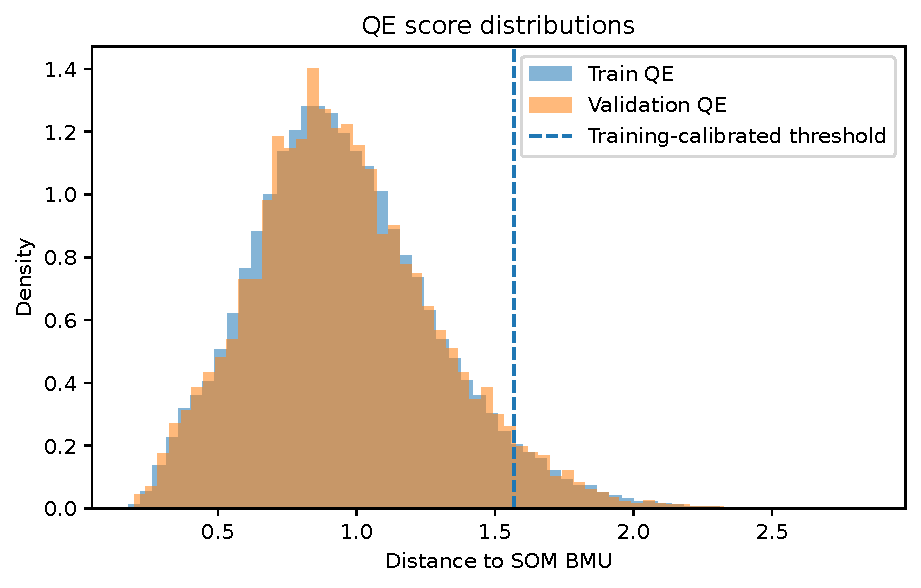
\includegraphics[width=0.80\linewidth]{fig/qe_novelty_detection/qe_score_distribution.pdf}
\caption{Previously generated training and validation QE distributions with the frozen training-percentile threshold. This figure is not an OOD performance comparison.}\label{fig:qe}
\end{figure}

\subsection{U-Matrix and Comparison Methods}
For unit $j$ with grid neighbors $\mathcal N(j)$, a neighborhood-distance summary is
\begin{equation}
 U_j=\frac{1}{|\mathcal N(j)|}\sum_{k\in\mathcal N(j)}\lVert w_j-w_k\rVert_2.
\end{equation}
The example-level U-Matrix signal uses the score of an example's BMU neighborhood. It measures prototype-to-prototype separation, not necessarily distance of the example from its BMU. The original historical five-method SVHN comparison additionally includes Isolation Forest, One-Class SVM and feature autoencoder reconstruction error. Subsequent comparisons add MSP, energy, Mahalanobis and $k$-nearest-neighbor distance on the frozen CNN representation. Different historical fitting budgets remain documented limitations rather than being silently equalized.

\begin{figure}[htbp]\centering
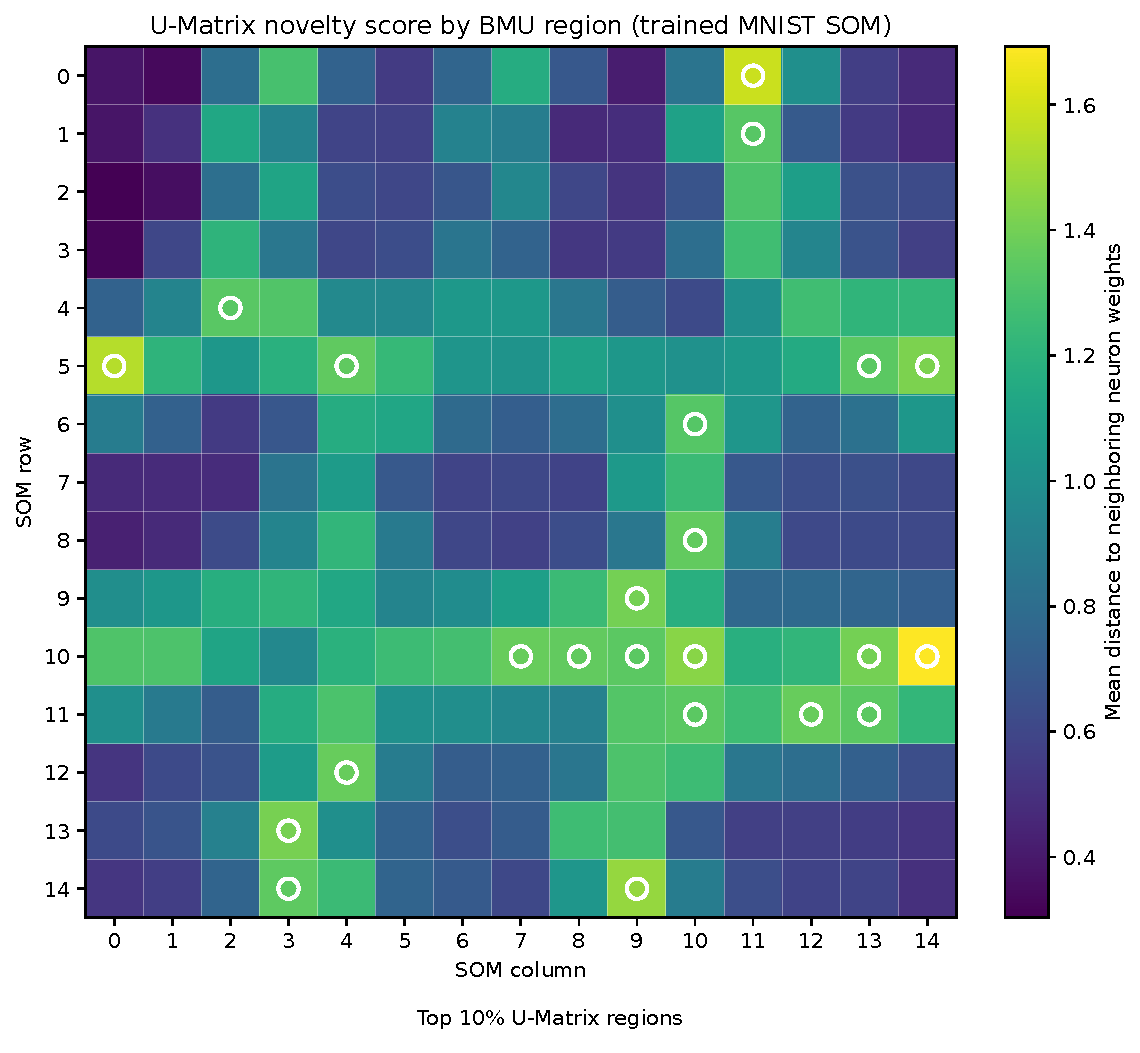
\includegraphics[width=0.84\linewidth]{fig/u_matrix_analysis/u_matrix_novelty_som_grid.pdf}
\caption{Recorded U-Matrix overview for the $15\times15$ SOM. Larger local prototype separations do not by themselves prove that individual samples are OOD.}\label{fig:umatrix}
\end{figure}

\section{Quantitative Evaluation}
We report AUROC as a threshold-independent ranking measure. AUPR uses OOD as the positive class and depends on class prevalence. FPR@95TPR denotes the minimum observed ROC false-positive rate at an operating point with TPR at least $0.95$; it must not be confused with the false-positive rate at the previously frozen QE threshold \parencite{fawcett2006roc,saito2015pr}. We do not use observed external-OOD results to change historical model settings.

\subsection{Primary MNIST versus Fashion-MNIST comparison}
The evaluation uses $10{,}500$ MNIST validation negatives and $10{,}000$ Fashion-MNIST test positives. The published point estimates and 95\% percentile bootstrap AUROC intervals below are from the recorded frozen-model evaluation with 2,000 stratified bootstrap iterations and seed 2026.
\begin{table}[htbp]\centering\small
\caption{Fashion-MNIST OOD ranking against MNIST validation. The intervals reflect resampling uncertainty for a fixed representation, not multi-seed training variation.}\label{tab:fashion}
\begin{tabular}{@{}lcc@{}}\toprule
Method & AUROC & 95\% bootstrap CI\\\midrule
Energy & 0.995678 & [0.995057, 0.996299]\\
MSP & 0.988127 & [0.986964, 0.989391]\\
$k$NN & 0.939197 & [0.935631, 0.942673]\\
Quantization Error & 0.918486 & [0.914368, 0.922389]\\
Mahalanobis & 0.733506 & [0.725800, 0.741031]\\
\bottomrule\end{tabular}
\end{table}
The measured Fashion-MNIST comparison shows that energy and MSP provide stronger AUROC than QE for the evaluated frozen CNN. Thus QE must not be characterized as the best overall detector. Separate evaluation details and reproducibility evidence are preserved in run-specific small metrics files rather than overwritten historical records.

\subsection{Historical SVHN comparison}
The original five-method benchmark uses the same $10{,}500$ MNIST validation examples and $26{,}032$ SVHN test examples, with the frozen MNIST representation. The table below records the historical benchmark; it is not retroactively merged into a single equal-budget experiment with the newer methods.
\begin{table}[htbp]\centering\small
\caption{Historical SVHN benchmark (one recorded seed). FPR@95TPR values are proportions, not percentages.}\label{tab:svhn}
\begin{tabular}{@{}lccc@{}}\toprule
Method & AUROC & AUPR & FPR@95TPR\\\midrule
QE & 0.9811 & 0.9766 & 0.0453\\
U-Matrix & 0.9696 & 0.9865 & 0.0701\\
Isolation Forest & 0.2383 & 0.5552 & 0.8718\\
One-Class SVM & 0.9604 & 0.9764 & 0.1794\\
Feature autoencoder & 0.0077 & 0.4979 & 0.9999\\
\bottomrule\end{tabular}
\end{table}
At the historical frozen QE threshold, the recorded detector flagged 25,036 of 26,032 SVHN cases (96.17\% detection) and exceeded the threshold for 5.13\% of MNIST validation. These two figures describe one fixed threshold, whereas the AUROC and FPR@95TPR results above evaluate ranking or another operating point.

\subsection{Additional SVHN baselines}
Newer, separately recorded SVHN results provide energy AUROC 0.999797 (AUPR 0.999917), MSP AUROC 0.998495 (AUPR 0.999358), and Mahalanobis AUROC 0.776437 (AUPR 0.785875). These findings again show that energy and MSP outperform QE in this evaluated setting. Because historical model fitting budgets and experimental chronology differ, they should not be presented as a prospectively frozen all-method competition.

\section{U-Matrix Association and Failure Analysis}
Across 10,500 MNIST validation samples, QE and the U-Matrix BMU score have a recorded Spearman rank correlation of $0.4396$. The moderate association is consistent with related but distinct SOM geometry signals.
\begin{figure}[htbp]\centering
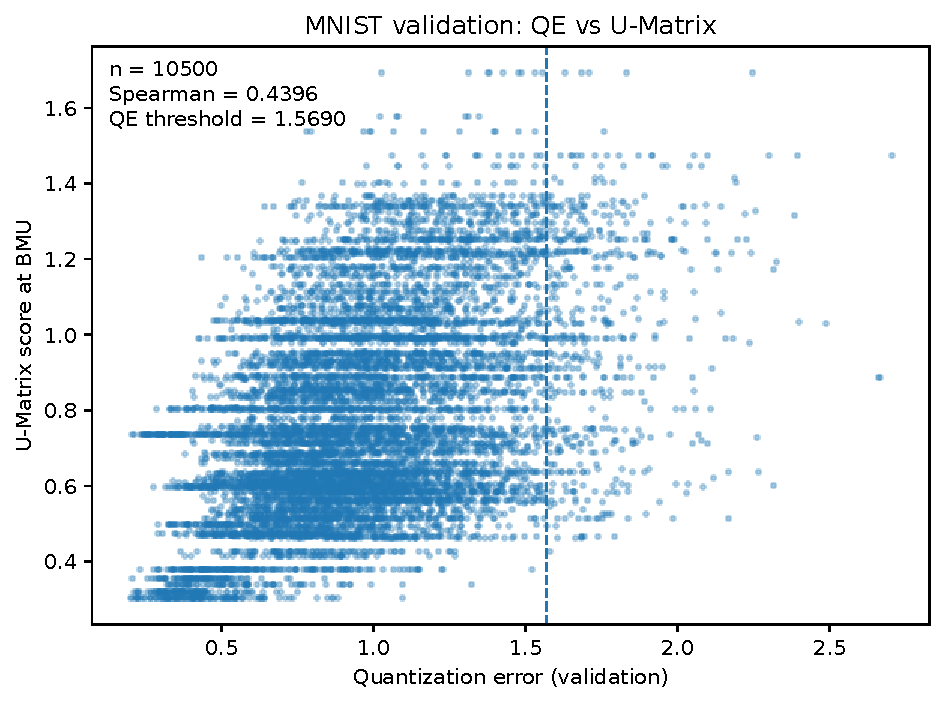
\includegraphics[width=0.82\linewidth]{fig/u_matrix_analysis/qe_u_matrix_validation_initial.pdf}
\caption{Recorded QE versus U-Matrix association on MNIST validation; the figure is a development-only comparison.}\label{fig:association}
\end{figure}
The historical QE experiment missed 996 SVHN samples at its frozen threshold. Several low-scoring examples have clean, MNIST-like numeral strokes; this visual pattern is a hypothesis about representation similarity, not a causal explanation. \paragraph{Unexpected baseline rankings and diagnostic status.}
The historical Isolation Forest (AUROC $0.2383$) and feature autoencoder (AUROC $0.0077$) fall substantially below the chance-level value of $0.5$ under the recorded score definitions (Table~\ref{tab:svhn}). This means that the recorded scores rank many evaluated ID/OOD pairs opposite to the desired ``larger means more novel'' ordering; it does \emph{not} by itself establish a programming error. Two possibilities requiring controlled investigation are anomaly-score orientation (including whether the library returns normality rather than anomaly scores) and inconsistent feature transformations between fitting and scoring, particularly in the historical autoencoder. A separate validation-only reproduction confirmed seven historical MNIST score/loss summaries (Section~6), but \emph{did not} recompute the SVHN AUROCs, audit score orientation on independent OOD labels, or recover the original autoencoder checkpoint. Therefore the cause has not been verified. We preserve the original AUROCs and do not flip signs, retune, or reinterpret the reported benchmark after inspecting the OOD outcomes. A future pre-specified diagnostic run should inspect score conventions, train/evaluation scaling, OOD-positive label assignment, and score distributions, saving new provenance and run identifiers.

\begin{figure}[htbp]\centering
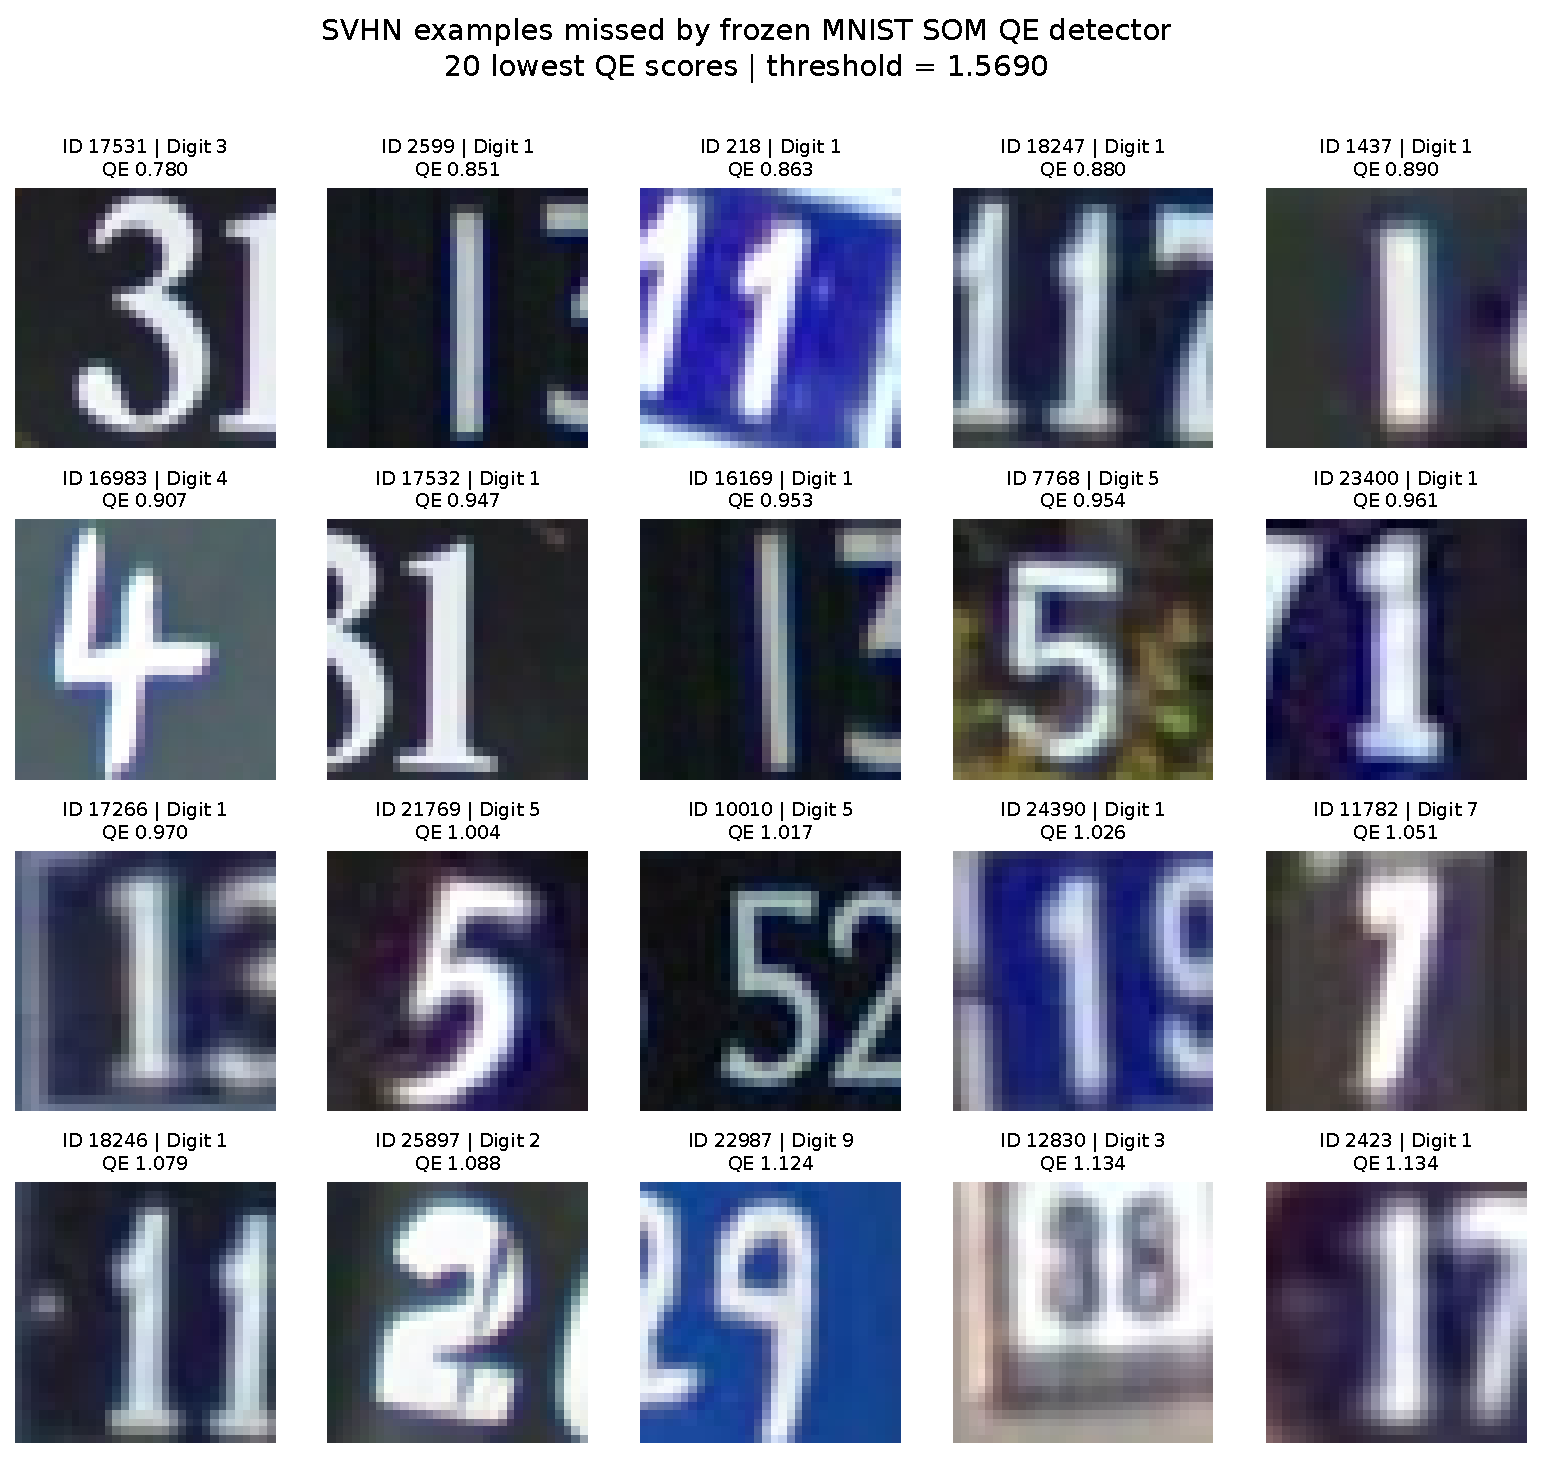
\includegraphics[width=0.90\linewidth]{fig/novelty_benchmark/qe_missed_svhn_examples.pdf}
\caption{Recorded lowest-QE SVHN examples missed at the original frozen threshold. These examples are descriptive, not a complete explanation of model behavior.}\label{fig:missed}
\end{figure}

\section{Leakage Control and Reproducibility}
The CNN and SOM were frozen for the documented Phase 3 comparisons. Training embeddings supplied model fitting and the training-derived QE threshold. MNIST validation supplied ID evaluation examples; the official MNIST final-test split was not used for the reported Phase 3 results. External Fashion-MNIST and SVHN test samples supplied observed OOD evaluation evidence, not inputs for post-hoc fitting or threshold selection. As these external sets have now been examined, further configuration changes using their outcomes would be exploratory and require a new protocol and run IDs; they must not be represented as independent validation.

The preregistration document's recorded writing date does not establish from Git history alone that its criteria were fixed before all external OOD results were examined. Historical JSON evidence has been preserved under run-specific directories with a relocation record. The latest EC2 verification completed 74 Phase 3 tests and 172 full MNIST tests successfully, with clean Phase 3 Ruff checks; the earlier Phase 1 data-path errors were resolved by running the suite from the appropriate working directory without changing Phase 1 code. SHA-256 input provenance and run-ID overwrite preflight remain part of the verification procedure.

A separate, newly identified verification run (\texttt{mnist\_historical\_baseline\_verification\_s42\_v1}) reproduced all seven historical MNIST-validation summary measurements with zero absolute numerical difference: Isolation Forest and One-Class SVM score means and standard deviations, and the feature autoencoder initial loss, final loss and mean validation reconstruction error. Frozen training and validation embedding SHA-256 fingerprints matched the references. This verification used MNIST training/validation evidence only; its seven comparisons are summary statistics, not a rerun of the full SVHN discrimination experiment. This supports numerical agreement under the currently committed settings, not byte-identical regeneration of the original historical JSON, checkpoint, or execution environment. The original autoencoder checkpoint and historical package-version manifest remain unavailable; old metrics were not overwritten. No final MNIST test or external OOD samples were accessed during this validation-only reproduction.

\section{Limitations and Interpretation}
This draft reports fixed-model bootstrap sampling intervals but not variation across at least five independent training seeds. The original One-Class SVM used 10,000 MNIST training embeddings whereas some other fitted baselines used 49,000. The cause of the historical autoencoder score behavior and the below-chance Isolation Forest ranking remains unresolved; orientation, consistent preprocessing, and positive-label definitions require a prospective diagnostic evaluation. The separate seven-summary reproduction does not validate the original SVHN AUROCs or establish an identical historic environment. No final locked MNIST test-set result is claimed. The comparison demonstrates useful novelty ranking on the examined distributions, not universal or clinically transferable OOD behavior.

\section{Conclusion and Next Phase}
The principal Fashion-MNIST comparison finds energy and MSP above SOM QE in AUROC, with QE still providing a meaningful prototype-distance novelty signal. The historical SVHN benchmark shows strong QE discrimination relative to its original comparison set, while additional SVHN baselines surpass QE. A future protocol-compliant study should equalize fitting budgets, examine multiple seeds and controls, resolve historical reproduction gaps, and fix the final selection rules before using the untouched MNIST final-test split. These Phase 3 outputs can inform the project's subsequent guided-retraining work without prematurely claiming final benchmark success.

\printbibliography[title={References}]
\end{document}
